\documentclass{article}

\usepackage{times}
\usepackage[left=1in,right=1in,top=1in,bottom=1in]{geometry}
\usepackage{enumitem}
\usepackage{amsmath}
\usepackage{amssymb}
\usepackage{tikz}

\title{Maths}
\author{Alexander}
\date{\today}

\begin{document}
\maketitle
\section*{Precalculus}

\subsection*{Composite and inverse functions}



\subsection*{Trigonometry}

\begin{center}
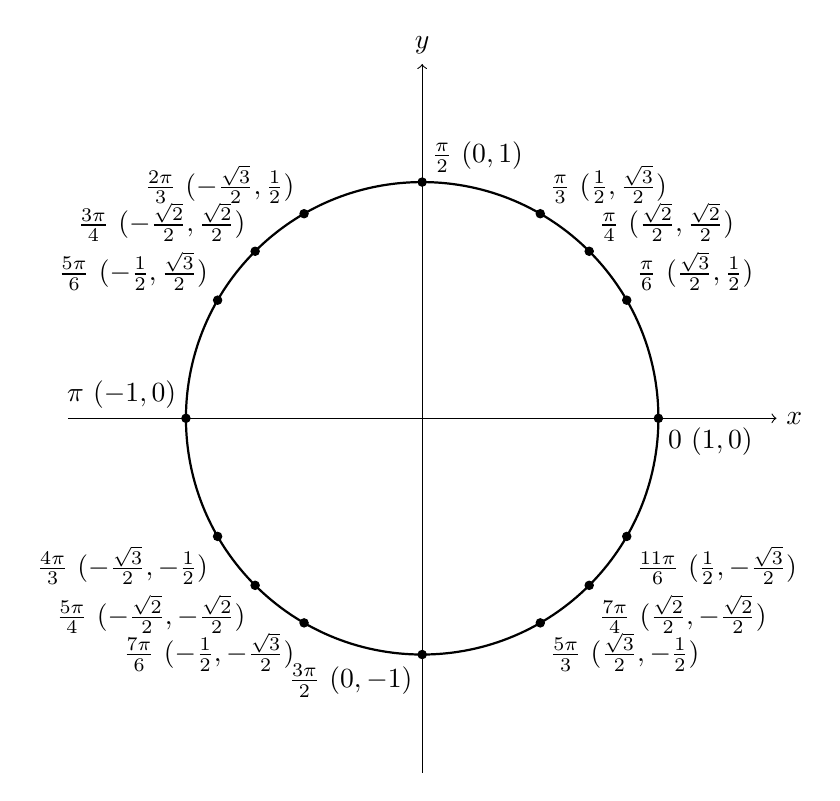
\begin{tikzpicture}
  	% Draw the enlarged unit circle
	\draw[thick] (0,0) circle [radius=3cm];
  
  	% Draw the axes
	\draw[->] (-4.5,0) -- (4.5,0) node[right] {$x$};
	\draw[->] (0,-4.5) -- (0,4.5) node[above] {$y$};
  
	% Label the key points
  	\filldraw (3,0) circle (1.5pt) node[below right] {$0$ $(1,0)$}; % Q1
  	\filldraw ({3*cos(30)},{3*sin(30)}) circle (1.5pt) node[above right] {$\frac{\pi}{6}$ $(\frac{\sqrt{3}}{2}, \frac{1}{2})$}; % Q1
  	\filldraw ({3*cos(45)},{3*sin(45)}) circle (1.5pt) node[above right] {$\frac{\pi}{4}$ $(\frac{\sqrt{2}}{2}, \frac{\sqrt{2}}{2})$}; % Q1
	\filldraw ({3*cos(60)},{3*sin(60)}) circle (1.5pt) node[above right] {$\frac{\pi}{3}$ $(\frac{1}{2}, \frac{\sqrt{3}}{2})$}; % Q1
  
	\filldraw (0,3) circle (1.5pt) node[above right] {$\frac{\pi}{2}$ $(0,1)$}; % Q2
  	\filldraw ({3*cos(120)},{3*sin(120)}) circle (1.5pt) node[above left] {$\frac{2\pi}{3}$ $(-\frac{\sqrt{3}}{2}, \frac{1}{2})$}; % Q2
  	\filldraw ({3*cos(135)},{3*sin(135)}) circle (1.5pt) node[above left] {$\frac{3\pi}{4}$ $(-\frac{\sqrt{2}}{2}, \frac{\sqrt{2}}{2})$}; % Q2
  	\filldraw ({3*cos(150)},{3*sin(150)}) circle (1.5pt) node[above left] {$\frac{5\pi}{6}$ $(-\frac{1}{2}, \frac{\sqrt{3}}{2})$}; % Q2
  
  	\filldraw (-3,0) circle (1.5pt) node[above left] {$\pi$ $(-1, 0)$}; % Q3
  	\filldraw ({3*cos(210)},{3*sin(210)}) circle (1.5pt) node[below left] {$\frac{4\pi}{3}$ $(-\frac{\sqrt{3}}{2}, -\frac{1}{2})$}; % Q3
  	\filldraw ({3*cos(225)},{3*sin(225)}) circle (1.5pt) node[below left] {$\frac{5\pi}{4}$ $(-\frac{\sqrt{2}}{2}, -\frac{\sqrt{2}}{2})$}; % Q3
  	\filldraw ({3*cos(240)},{3*sin(240)}) circle (1.5pt) node[below left] {$\frac{7\pi}{6}$ $(-\frac{1}{2}, -\frac{\sqrt{3}}{2})$}; % Q3
  
  	\filldraw (0,-3) circle (1.5pt) node[below left] {$\frac{3\pi}{2}$ $(0, -1)$}; % Q4
  	\filldraw ({3*cos(300)},{3*sin(300)}) circle (1.5pt) node[below right] {$\frac{5\pi}{3}$ $(\frac{\sqrt{3}}{2}, -\frac{1}{2})$}; % Q4
  	\filldraw ({3*cos(315)},{3*sin(315)}) circle (1.5pt) node[below right] {$\frac{7\pi}{4}$ $(\frac{\sqrt{2}}{2}, -\frac{\sqrt{2}}{2})$}; % Q4
  	\filldraw ({3*cos(330)},{3*sin(330)}) circle (1.5pt) node[below right] {$\frac{11\pi}{6}$ $(\frac{1}{2}, -\frac{\sqrt{3}}{2})$}; % Q4
\end{tikzpicture}
\end{center}

\begin{enumerate} 
	\item Pythagorean:
		\begin{itemize}
			\item $\sin^2(x) + \cos^2(x) = 1 $
			\item $\tan^2(x) + 1 = sec^2(x)$
			\item $1 + \cot^2(x) = csc^2(x)$
		\end{itemize}
	\item Reciprocal:
		\begin{itemize}
			\item $\csc(x) = \frac{1}{\sin(x)}$
			\item $\sec(x) = \frac{1}{\cos(x)}$
			\item $\cot(x) = \frac{1}{\tan(x)}$
		\end{itemize}
	\item Even-Odd:
		\begin{itemize}
			\item $\sin(-x) = -\sin(x)$
			\item $\cos(-x) = \cos(x)$
			\item $\tan(-x) = -\tan(x)$
		\end{itemize}
	\item Co-function:
		\begin{itemize}
			\item $\sin(\frac{\pi}{2}-x) = \cos(x)$
			\item $\cos(\frac{\pi}{2}-x) = \sin(x)$
			\item $\tan(\frac{\pi}{2}-x) = \cot(x)$
		\end{itemize}
	\item Double-Angle:
		\begin{itemize}
			\item $\sin(2x) = 2\sin(x)\cos(x)$
			\item $\cos(2x) = \cos^2(x) - \sin^2(x)$
			\item $\tan(2x) = \frac{2\tan(x)}{1-\tan^2(x)}$
		\end{itemize}
	\item Sum and Difference:
		\begin{itemize}
			\item $\sin(x \pm y) = \sin(x)\cos(y) \pm \cos(x)\sin(y)$
			\item $\cos(x \pm y) = \cos(x)\cos(y) \pm \sin(x)\sin(y)$
			\item $\tan(x \pm y) = \frac{\tan(x)\pm\tan(y)}{1\pm\tan(x)\tan(y)}$
		\end{itemize}
\end{enumerate}
	
\subsection*{Complex numbers}
\subsection*{Rational functions}
\subsection*{Conic sections}
\subsection*{Vectors}
\subsection*{Matrices}
\subsection*{Probability and combinatorics}
\subsection*{Series}
\subsection*{Limits and continuity}

\section*{Calculus}

	
\end{document}
